%% Copyright 2005 G. W. Knor
%%This work may be distributed and/or modified under the
% conditions of the LaTeX Project Public License, either version 1.3
% of this license or (at your option) any later version.
% The latest version of this license is in
% http://www.latex-project.org/lppl.txt
% and version 1.3 or later is part of all distributions of LaTeX
% version 2005/12/01 or later.
%%This work has the LPPL maintenance status "maintained".
%%The Current Maintainer of this work is G. W. Knor.

\documentclass{beamer}
\usepackage{graphicx}
\usepackage{sidecap}
\usepackage{courier}
\usepackage{listings}
\usepackage{hyperref}
\usepackage[utf8]
{inputenc}
\lstset{
    breaklines=true,
    breakatwhitespace=true,
    postbreak=\raisebox{0ex}[0ex][0ex]{\ensuremath{\color{red}\hookrightarrow\space}}
}
\setcounter{tocdepth}{1}

\definecolor{keywords}{RGB}{255,0,90}
\definecolor{comments}{RGB}{0,0,113}
\definecolor{red}{RGB}{160,0,0}
\definecolor{green}{RGB}{0,150,0}

\lstset{language=Python,
        basicstyle=\ttfamily\small,
        keywordstyle=\color{keywords},
        commentstyle=\color{comments},
        stringstyle=\color{red},
        showstringspaces=false,
        identifierstyle=\color{green}}

\title{Common programming mistakes}
\author{Dariusz Śmigiel}
\date{PyCon PL 2014: 18.10.2014}
\usetheme{Madrid}
\usecolortheme{seahorse}

\begin{document}

\begin{frame}
\titlepage
\end{frame}

\section*{Laptop}
\begin{frame}
    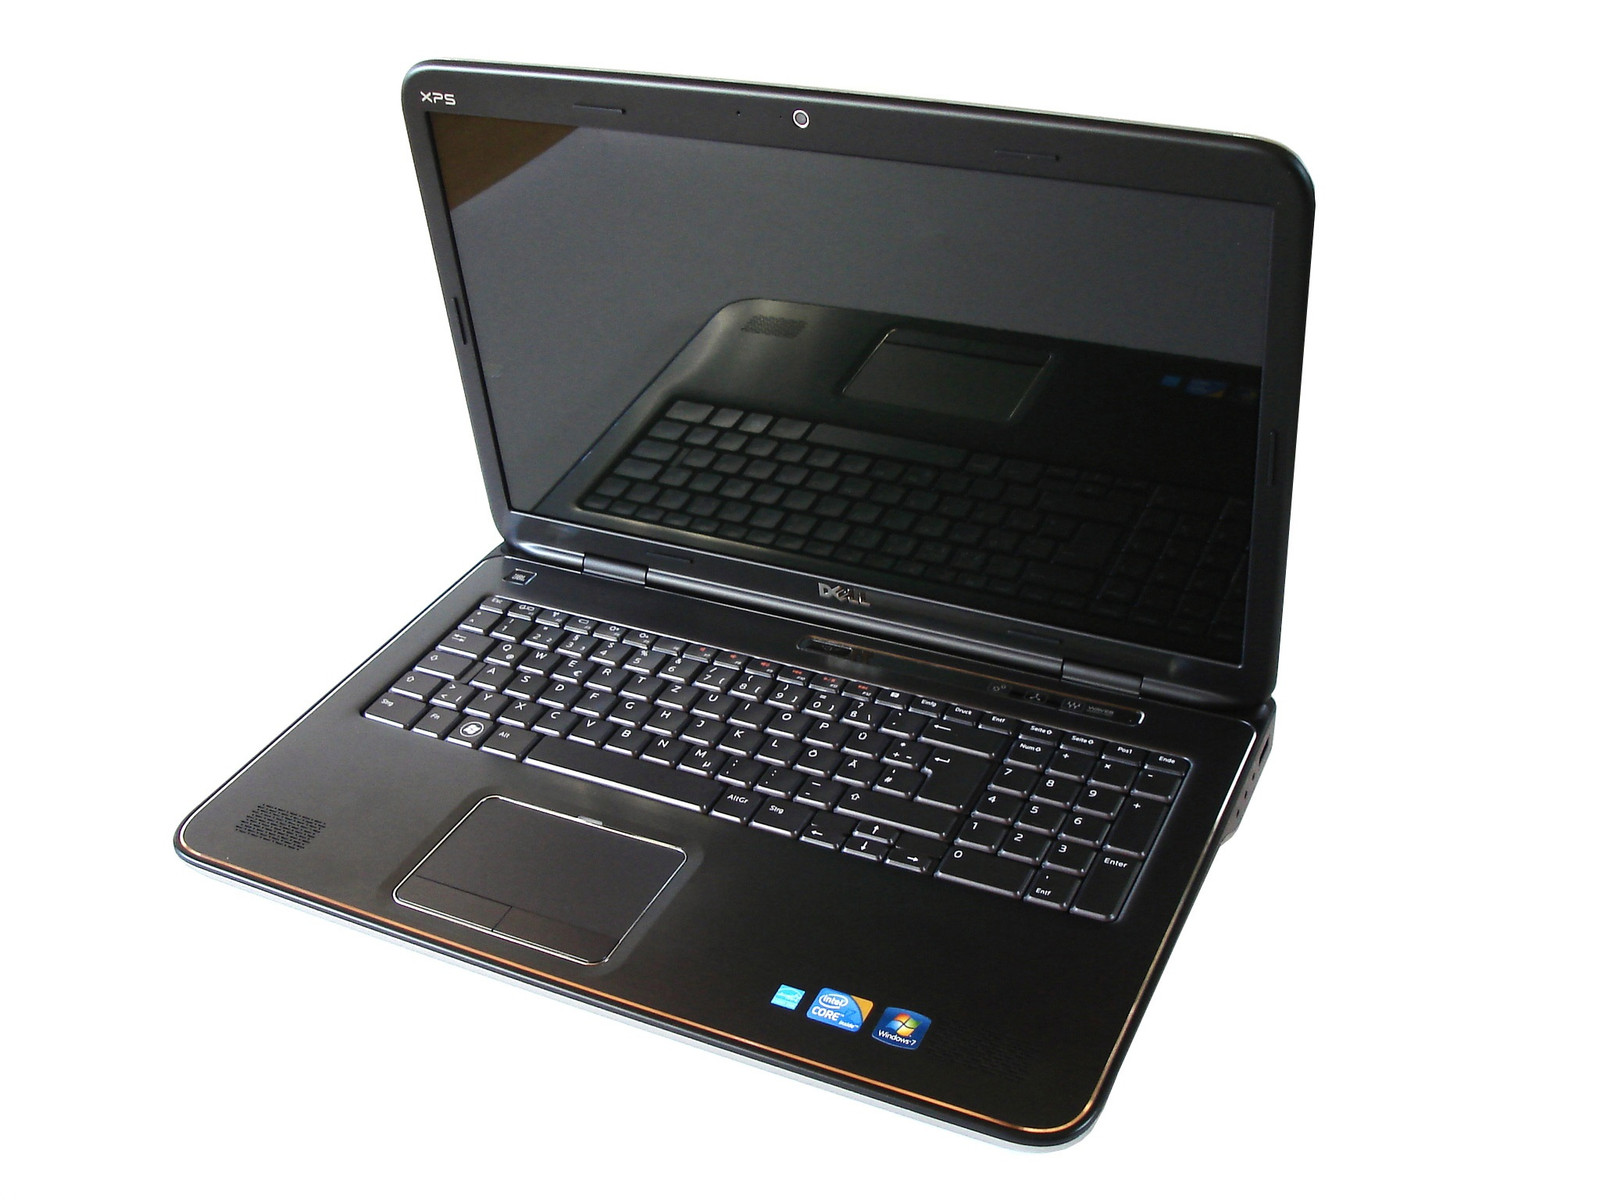
\includegraphics[width=1\textwidth]{images/dell_xps.jpg}
\end{frame}

\section*{Full Disclosure}
\begin{frame}
Based on Martin Chikilian:\\
\url{www.toptal.com/python/top-10-mistakes-that-python-programmers-make}
\end{frame}

\section*{Outline}
\begin{frame}
\tableofcontents
\end{frame}

\section{Question?!}

\begin{frame}
\begin{center}
    \structure{\insertsection}
\end{center}
Let any one of you who is without sin be the first to throw a stone at her.
\end{frame}
\begin{frame}
    \begin{center}
        
\includegraphics[width=1\textwidth]{images/stone1.jpg}
    \end{center}
\end{frame}


\section{Function arguments}
\subsection{Current behaviour}
\begin{frame}
\begin{center}
\structure{\insertsection}
\end{center}
\lstinputlisting[language=Python, firstline=14, lastline=16]{text.md}
\pause
\lstinputlisting[language=Python, firstline=27, lastline=28]{text.md}
\end{frame}
\begin{frame}
\lstinputlisting[language=Python, firstline=29, lastline=30]{text.md}
\pause
\begin{center}

\includegraphics[width=0.5\textwidth]{images/surprised1.png}
\end{center}
\pause
\lstinputlisting[language=Python, firstline=31, lastline=32]{text.md}
\pause
\begin{center}

\includegraphics[width=0.5\textwidth]{images/surprised2.png}
\end{center}
\end{frame}

\subsection{What's happening}
\begin{frame}
Early binding \\
\begin{itemize}
    \item initialization on function definition;
    \item by purpose: compiler associates identifier name (function or variable) with machine address
\end{itemize}
\end{frame}

\subsection{Solution}
\begin{frame}
\lstinputlisting[language=Python, firstline=40, lastline=44]{text.md}
\pause \lstinputlisting[language=Python, firstline=46, lastline=49]{text.md}
\end{frame}

\subsection{Comparison}
\begin{frame}[fragile]
\begin{lstlisting}
    >>> def foo(bar=[]):
    ...     bar.append("baz")
    ...     return bar
\end{lstlisting}
\begin{lstlisting}
  3           0 LOAD_FAST                0 (bar)
              3 LOAD_ATTR                0 (append)
              6 LOAD_CONST               1 ('baz')
              9 CALL_FUNCTION            1
             12 POP_TOP

  4          13 LOAD_FAST                0 (bar)
             16 RETURN_VALUE

\end{lstlisting}
\end{frame}
\begin{frame}[fragile]
\begin{lstlisting}
    >>> def foo(bar=None):
    ...     if bar is None:
    ...         bar = []
    ...     bar.append("baz")
    ...     return bar
\end{lstlisting}
\begin{lstlisting}
  7           0 LOAD_FAST                0 (bar)
              3 POP_JUMP_IF_TRUE        15

  8           6 BUILD_LIST               0
              9 STORE_FAST               0 (bar)
             12 JUMP_FORWARD             0 (to 15)

  9     >>   15 LOAD_FAST                0 (bar)
             18 LOAD_ATTR                0 (append)
             21 LOAD_CONST               1 ('baz')
             24 CALL_FUNCTION            1
             27 POP_TOP

 10          28 LOAD_FAST                0 (bar)
             31 RETURN_VALUE

\end{lstlisting}
\end{frame}


\section{Binding variables in closures}
\subsection{Current behaviour}

\begin{frame}
    \begin{center}
        \structure{\insertsection}
    \end{center}

    \lstinputlisting[language=Python, firstline=54, lastline=58]{text.md}
    \pause

    \begin{columns}
        \begin{column}{0.48\textwidth}
            \lstinputlisting[language=Python, firstline=71, lastline=75]{text.md}
        \end{column}
        \begin{column}{0.48\textwidth}
            
\includegraphics[width=0.48\textwidth]{images/facepalm.jpg}
        \end{column}
    \end{columns}
\end{frame}

\subsection{What's happening}
\begin{frame}
Late binding \\
\begin{itemize}
\item values of variables in closures are looked up at the time the inner function is called;
\item by then, loop has completed and \texttt{i} returns 4
\end{itemize}
\end{frame}

\subsection{Solution}
\begin{frame}
        \lstinputlisting[language=Python, firstline=103, lastline=109]{text.md}
        \pause
    \begin{columns}
        \begin{column}{0.48\textwidth}
            \lstinputlisting[language=Python, firstline=110, lastline=115]{text.md}
        \end{column}
        \begin{column}{0.48\textwidth}
            \pause
            
\includegraphics[width=0.48\textwidth]{images/ok.jpg}
        \end{column}
    \end{columns}
\end{frame}

\subsection{Better idea}
\begin{frame}
\lstinputlisting[language=Python, firstline=119, lastline=134]{text.md}
\end{frame}

\section{Local names}
\subsection{Current behaviour}
\begin{frame}[fragile]
\begin{center}
\structure{\insertsection}
\end{center}
    \begin{lstlisting}
    x = 99
    >>> def func():
    ...     print(x)
    ...
    ...
    >>> func()
    99
    \end{lstlisting}
\end{frame}

\begin{frame}
\begin{center}
\structure{\insertsection}
\end{center}
\lstinputlisting[language=Python, firstline=139, lastline=143]{text.md}
\pause \lstinputlisting[language=Python, firstline=148, lastline=152]{text.md}
\end{frame}

\subsection{What's happening}
\begin{frame}
Local names \\
\begin{itemize}
\item Python sees the assignment to \texttt{x}
\item it's decided that \texttt{x} is a local variable in function
\item when function is run, assignment hasn't yet happened
\item Python raises undefined error
\end{itemize}
\end{frame}

\subsection{Solution}
\begin{frame}
\lstinputlisting[language=Python, firstline=160, lastline=165]{text.md}
\pause \lstinputlisting[language=Python, firstline=166, lastline=167]{text.md}
\end{frame}

\section{Scope rules}
\subsection{Current behaviour}
\begin{frame}
\begin{center}
\structure{\insertsection}
\end{center}
\lstinputlisting[language=Python, firstline=247, lastline=251]{text.md}
\pause \lstinputlisting[language=Python, firstline=256, lastline=260]{text.md}
\end{frame}

\subsection{What's happening}
\begin{frame}
Python scope resolution is based on \texttt{LEGB}:
\begin{itemize}
\item Local - names assigned in any way within a function (\texttt{def} or \texttt{lambda}) and not declared global in that function;
\item Enclosing function locals - name in the local	scope of any and all enclosing (\texttt{def} or \texttt{lambda}), from inner to outer;
\item Global (module) - names assigned at the top-level of a module file, or declared global in a \texttt{def} within the file;
\item Built-in (Python) - names preassigned in a built-in names module: \texttt{open}, \texttt{range}, \texttt{SyntaxError}, ...
\end{itemize}
So, when you make an assignment to variable, Python considers it as in local scope.
It shadows everything, that is outside this scope. In this case, we don't "see"
variable \texttt{i} declared before function definition.
\end{frame}

\subsection{Solution}
\begin{frame}
\lstinputlisting[language=Python, firstline=278, lastline=282]{text.md}
\pause \lstinputlisting[language=Python, firstline=283, lastline=286]{text.md}
\pause
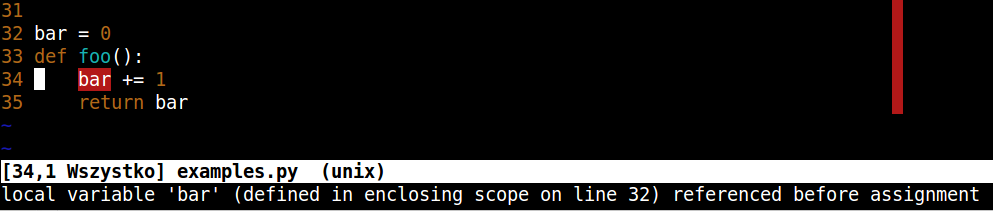
\includegraphics[width=1\textwidth]{images/scope.png}
\end{frame}

\section{Class variables}
\subsection{Current behaviour}
\begin{frame}[fragile]
\begin{center}
\structure{\insertsection}
\end{center}
\lstinputlisting[language=Python, firstline=172, lastline=179]{text.md}
\pause \lstinputlisting[language=Python, firstline=185, lastline=186]{text.md}
\pause \lstinputlisting[language=Python, firstline=190, lastline=190]{text.md}
\pause \lstinputlisting[language=Python, firstline=191, lastline=192]{text.md}
\pause \lstinputlisting[language=Python, firstline=196, lastline=196]{text.md}
\pause \lstinputlisting[language=Python, firstline=197, lastline=198]{text.md}
\end{frame}
\begin{frame}
    \begin{center}
        
\includegraphics[width=1\textwidth]{images/why.png}
    \end{center}
\end{frame}
\subsection{What's happening}
\begin{frame}
MRO: Method Resolution Order \\
\begin{itemize}
\item class B and C inherite from A
\item all 3 classes have the same value of \texttt{x}
\item \texttt{x} in B class, overrides the same property in A
\item modifying \texttt{x} in A class, we have the same value for A and C classes
\end{itemize}
\end{frame}

\subsection{Solution}
\begin{frame}[fragile]
Remember about it ;) \\
\pause
or compute:
\begin{lstlisting}
L[A] = A O
L[B] = B A
L[C] = C A

L[C] = C + merge(A, O) = C A O
\end{lstlisting}
\pause
or use \texttt{mro()} method:
\begin{lstlisting}
A.mro()
[<class '__main__.A'>, <type 'object'>]
B.mro()
[<class '__main__.B'>, <class '__main__.A'>, <type 'object'>]
C.mro()
[<class '__main__.C'>, <class '__main__.A'>, <type 'object'>]
\end{lstlisting}
\end{frame}

\section{Exception handling}
\subsection{Current behaviour}
\begin{frame}
\begin{center}
\structure{\insertsection}
\end{center}
\lstinputlisting[language=Python, firstline=208, lastline=212]{text.md}
\pause \lstinputlisting[language=Python, firstline=219, lastline=221]{text.md}
\end{frame}

\subsection{What's happening}
\begin{frame}
Python 2
\begin{itemize}
\item old syntax  is supported for backwards compatibility
\item \texttt{except ValueError, e == except ValueError as e}
\item \texttt{except ValueError, IndexError == except ValueError as IndexError}
\end{itemize}
\end{frame}

\subsection{Solution}
\begin{frame}
\texttt{Python 2}
\lstinputlisting[language=Python, firstline=236, lastline=238]{text.md}
\pause \lstinputlisting[language=Python, firstline=239, lastline=240]{text.md}
\pause \texttt{Python 3}
\lstinputlisting[language=Python, firstline=231, lastline=232]{text.md}
\end{frame}

\section{Modifying list while iterating over it}
\subsection{Current behaviour}
\begin{frame}
\begin{center}
\structure{\insertsection}
\end{center}
\lstinputlisting[language=Python, firstline=291, lastline=296]{text.md}
\pause \lstinputlisting[language=Python, firstline=297, lastline=299]{text.md}
\end{frame}

\subsection{What's happening}
\begin{frame}
Iterating
\begin{itemize}
\item iterate over the list
\item remove odd values
\item list is shrinking
\item list is shorter than expected
\end{itemize}
\end{frame}

\subsection{Solution?}
\begin{frame}
\lstinputlisting[language=Python, firstline=307, lastline=314]{text.md}
\pause
\begin{center}

\includegraphics[width=0.5\textwidth]{images/nope.jpg}
\end{center}
\end{frame}
\begin{frame}
\lstinputlisting[language=Python, firstline=318, lastline=326]{text.md}
\end{frame}

\subsection{Better idea}
\begin{frame}
\lstinputlisting[language=Python, firstline=331, lastline=335]{text.md}
\end{frame}

\section{Name clashing with Python Standard Library modules}
\subsection{Current behaviour}
\begin{frame}
\begin{center}
\structure{\insertsection}
\end{center}
\lstinputlisting[language=Python, firstline=340, lastline=343]{text.md}
\pause \texttt{sender.py}
\lstinputlisting[language=Python, firstline=347, lastline=352]{text.md}
\pause \lstinputlisting[language=Python, firstline=357, lastline=359]{text.md}
\end{frame}

\subsection{What's happening}
\begin{frame}
Standard Library
\begin{itemize}
\item import PSL \texttt{email}
\item use functions from this module
\item wonder, why is imported local, than expected one.
\end{itemize}
\end{frame}

\subsection{Solution}
\begin{frame}
Python uses pre-defined order of importing modules. When we're trying to import \texttt{spam} it looks in:
\begin{enumerate}
\item built-in module (string, re, datetime, etc.)
\item searches for a file named \texttt{spam.py} in directories given by the variable \texttt{sys.path} in
\begin{itemize}
\item the directory containing the input script (or the current directory).
\item PYTHONPATH (a list of directory names, with the same syntax as the shell variable PATH).
\item the installation-dependent default.
\end{itemize}
\end{enumerate}
\end{frame}

\section{Bonus Mistake: Differences between Python 2 and Python 3}
\subsection{Current behaviour}
\begin{frame}
\begin{center}
\structure{\insertsection}
\end{center}
\lstinputlisting[language=Python, firstline=376, lastline=394]{text.md}
\end{frame}
\begin{frame}
\texttt{Python 2}
\lstinputlisting[language=Python, firstline=399, lastline=404]{text.md}
\pause \texttt{Python 3}
\lstinputlisting[language=Python, firstline=408, lastline=415]{text.md}
\end{frame}

\subsection{What's happening}
\begin{frame}
When an exception has been assigned to a variable name using \texttt{as target}, it is cleared at the end of the except clause:
\lstinputlisting[language=Python, firstline=420, lastline=424]{text.md}
\end{frame}

\subsection{Solution}
\begin{frame}[fragile]
\begin{lstlisting}
    import sys

    def bar(i):
        if i == 1:
            raise KeyError(1)
        if i == 2:
            raise ValueError(2)
\end{lstlisting}
\end{frame}
\begin{frame}[fragile]
\begin{lstlisting}
    def good():
        exception = None
        try:
            bar(int(sys.argv[1]))
        except KeyError as e:
            exception = e
            print('key error')
        except ValueError as e:
            exception = e
            print('value error')
        print(exception)

    good()
\end{lstlisting}
\pause
\begin{lstlisting}
    $ python3 foo.py 1
    key error
    1
    $ python3 foo.py 2
    value error
    2
\end{lstlisting}
\end{frame}


\section*{Summary}
\begin{frame}
\begin{center}
Thank you for your attention!
\end{center}
\end{frame}
\end{document}
